\documentclass{article}
\usepackage{graphicx}
\usepackage{color}
\usepackage{listings}
\usepackage{fullpage}
\usepackage[framed]{mcode}
\usepackage{amsmath}
\usepackage[utf8x]{inputenc}
\usepackage{import}
\usepackage{setspace}
\usepackage{subcaption}
\usepackage{hyperref}
\usepackage{float}
\usepackage{pdfpages}
\definecolor{lightgray}{gray}{0.5}
\setlength{\parindent}{0pt}
\usepackage{setspace} 
\setstretch{1.5}
\newcommand{\purple}[1]{\textcolor{purple}{#1}}

\date{May 7, 2020 (Extension)}

% Problem counter
\newcounter{number}
\setcounter{number}{1}

\begin{document}

	\title{BE 521 Final Report}
	\author{Team ECoG: Ikenna Achilihu and Sandy Tang}
	\maketitle
	\hrulefill

	\textbf{The Algorithm}

The algorithm we used for this BCI competition was to combine finger angle predictions from the linear regression (i.e. optimal decoder) model used in \textit{Kubanek et. Al}’s paper and weigh them by probability predictions from a logistic regression model in \textit{Chen et. Al}’s paper. In the pre-processing stage, we filtered each patient’s ECog data according to parameters in \textit{Kubanek et. Al}. We then calculated 9 features in the ECog data using a sliding window of 80 ms with an overlap of 40 ms (we describe our choice of features and engineering methods separately). After calculating the ECog feature (R) matrix shown in \textit{Warland et. Al}, we utilize the outputs of PCA to derive the principle components of the feature matrix that only contained components that explained 99\% of the variance. Training data and testing data were partitioned according to a 90/10 split, respectively. The feature matrix represented in PCA space was then used as an input into a linear regression model along with finger data (labels) to generate predictions for each subject’s 5 fingers, which were subsequently smoothed before correlating with ground truth. Shown in \textbf{getWindowedFeats.m}, this linear regression algorithm was used in parallel with logistic regression. Drawing inspiration from \textit{Chen et. al}, we then used a logistic regression model in order weight the aforementioned  linear regression predictions. Our training data input for logistic regression was the same ECog feature matrix described above. For the labels, we transformed the raw finger data labels into binary classifications (0 for no flexion, 1 for flexion), which were then smoothed. After training on the logistic regression model, the output probability predictions were smoothed once more and used to weight the linear regression predictions above to yield the final predictions. Based on competition data, our algorithm prediction accuracy was \underline{\textbf{0.5359}}. A detailed sequence of steps for our algorithm is as follows. A flow chart can be seen in \textbf{Figure 1}. \\


	\textbf{Detailed steps for linear regression}
	\begin{enumerate}
	    \item For filtering, we used MATLAB’s \textbf{filterDesigner} tool to design an FIR equiripple bandpass filter of order 100, with start frequency cutoffs of 0.15 Hz and 200 Hz, and stop frequency cutoffs of [0 Hz, 250 Hz] respectively. No channels were removed because including all channels did not change our accuracy.
	   
	    \item Calculate 9 features for Ecog data in all 3 subjects with \textbf{getWindowedFeats.m} and \textbf{get\_features.m}, \textbf{create\_R\_matrix.m} from \textit{Warland et. al}.
	    
        \begin{enumerate}
            \item Variance, Line Length, Average signal values, Haart Wavelet
            \item Bandpower in the following ranges: Beta (5- 15 Hz), Beta (20-25 Hz), Gamma (75 – 115 Hz), Gamma (125 – 160 Hz), Gamma (160 – 175 Hz)
            \item All features were z score normalized with respect to the training data
        \end{enumerate}
        
        \item Split feature matrix into testing and training data, 90/10.
        
        \item Input both training and testing data into \textbf{vis\_pcafeats.m} to reduce the dimensionality only down to components that explain 99\% of variance. This reduced dimensionality matrix now becomes our modified featured matrix.
        
        \item Input feature matrix into optimal linear decoder (linear regression) to return finger angle predictions. The labels were down-sampled at this point.
        
        \item Apply a moving average to all subjects’ up-sampled predictions given their high noise content \textbf{Figure 2}. In order to determine the ideal window size, we looped through a range of values that gave us the best accuracy. This window length for smoothing linear predictions was 3303 samples. The accuracy of this model alone was \underline{\textbf{0.4573}}, and the smoothed predictions can be seen in \textbf{Figure 3}.
        
        \item We chose not to do cross validation because of long computational times. Another reason for not performing cross validation is that, aside from posting on the leader board in comparison to our peers, there was no pressure to characterize the predictive performance of the models, nor to judge how they perform outside of the leader board data.\\
    \end{enumerate}

    \textbf{Detailed steps for logistic regression}
    \begin{enumerate}
        \item To further improve our accuracy from linear regression, we followed \textit{Chen et. al.}’s methodology in using a logistic regression. We use \textbf{classifyFinger.m} to classify the original finger angle labels as flexion (1) or no flexion (0). This was done through logical indexing for voltages above 1.5. 
        
        \item Smooth the finger angle labels by grouping all flexion spike trains within a 4 second window, which reduced the noise in the binary signal. This can be seen in \textbf{Figure 4}.
        
        \item Using the Ecog feature matrices as training data, and the smoothed binary classifications as labels, we trained a logistic regression model in \textbf{logfingModel.m}
        
        \item After getting the predictions as probability scores, we further smoothed these predictions using a moving average based on the same strategy used to smooth linear predictions.
        
        \item Final predictions were calculated by weighing the smoothed linear predictions by the smoothed probability scores and correlating this against ground truth. The final predictions are shown in \textbf{Figure 3}.\\
    \end{enumerate}
	\begin{minipage}{\linewidth}
        \centering
	    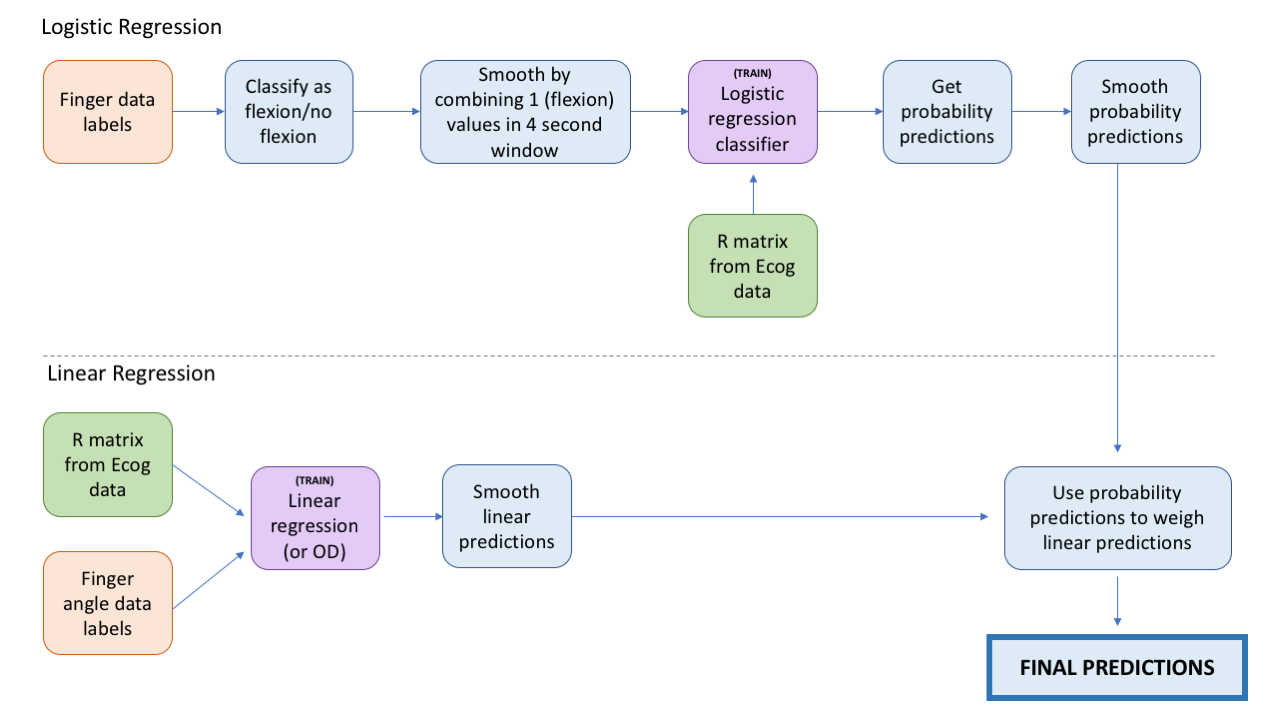
\includegraphics[scale=0.4]{flowchart.png}
	    \captionof{figure}{Flow chart of algorithm used for final competition.}
	    \label{fig1}
	\end{minipage}\\\\


    \textbf{Other methods tried}\\
    For feature engineering, we originally began with 14 features. In order to determine whether there was redundancy in our list of features, we wrote \textbf{get\_featuresHeat.m} and \textbf{getWindowedFeatsHeat.m} which returned z score normalized features per subjects, averaged across all of a subject’s respective channels. As seen in \textbf{Figure 5}, by creating a correlation matrix for each subject, we were able to discern that only 5 features might have been necessary. But to avoid eliminating crucial information through sheer trial and error, we drew inspiration from \textit{Chen et. al} to bring us to a total of 9 features before implementing PCA. We also tried Lasso as one of our feature selection methods, but found that the accuracy it gave us was not statistically different from our algorithm. Instead of trying too many different models, we focused on selecting an ideal set of features. Once we were able to get to at least \underline{\textbf{0.40}} accuracy with linear regression, we noticed the predictions were quite noisy. Starting out as a post-processing attempt to smooth our linear predictions, we realized we could combine our model with others, and \textit{Chen et. al} happened to work best.\\
    
\textbf{Comments on Finger Correlation}\\
One reason the ring finger was so correlated with the middle and pinky finger might be due to biomechanical connections between the fingers. Empirically, it has been shown that the thumb and index fingers are the most independent, whereas the middle and ring fingers are least dependent according to \textit{Hager-Ross and Schieber}. This makes sense because the index finger and thumb are used in highly specialized tasks, such as writing or gripping, and the ring finger tends to play a supportive role. Perhaps anatomy has adapted to this use both in how tissues and tendons are placed, but also how each finger is innervated to reflect this difference in use.\\

\textbf{Comments on Experience with Project}\\ 
This project definitely taught us that machine learning is part art, and part science. We needed to balance understanding enough about how a particular model works so that we could use it intelligently, but also not spend too much time on the details. Progress was also nonlinear, and we needed to backtrack often to problem solve what didn’t work- which means lots of our algorithm development was trial and error. Additionally, referring to research papers and replicating these methods was empowering given that this course is our introduction into machine learning. This reminded us that we don’t need to re-invent the wheel, and the challenge was creatively arranging and working upon the vast amount of research that already exists. Also, working on a project that can directly be translated into a device if we had time for hardware component was also exciting.\\

	\begin{minipage}{\linewidth}
        \centering
	    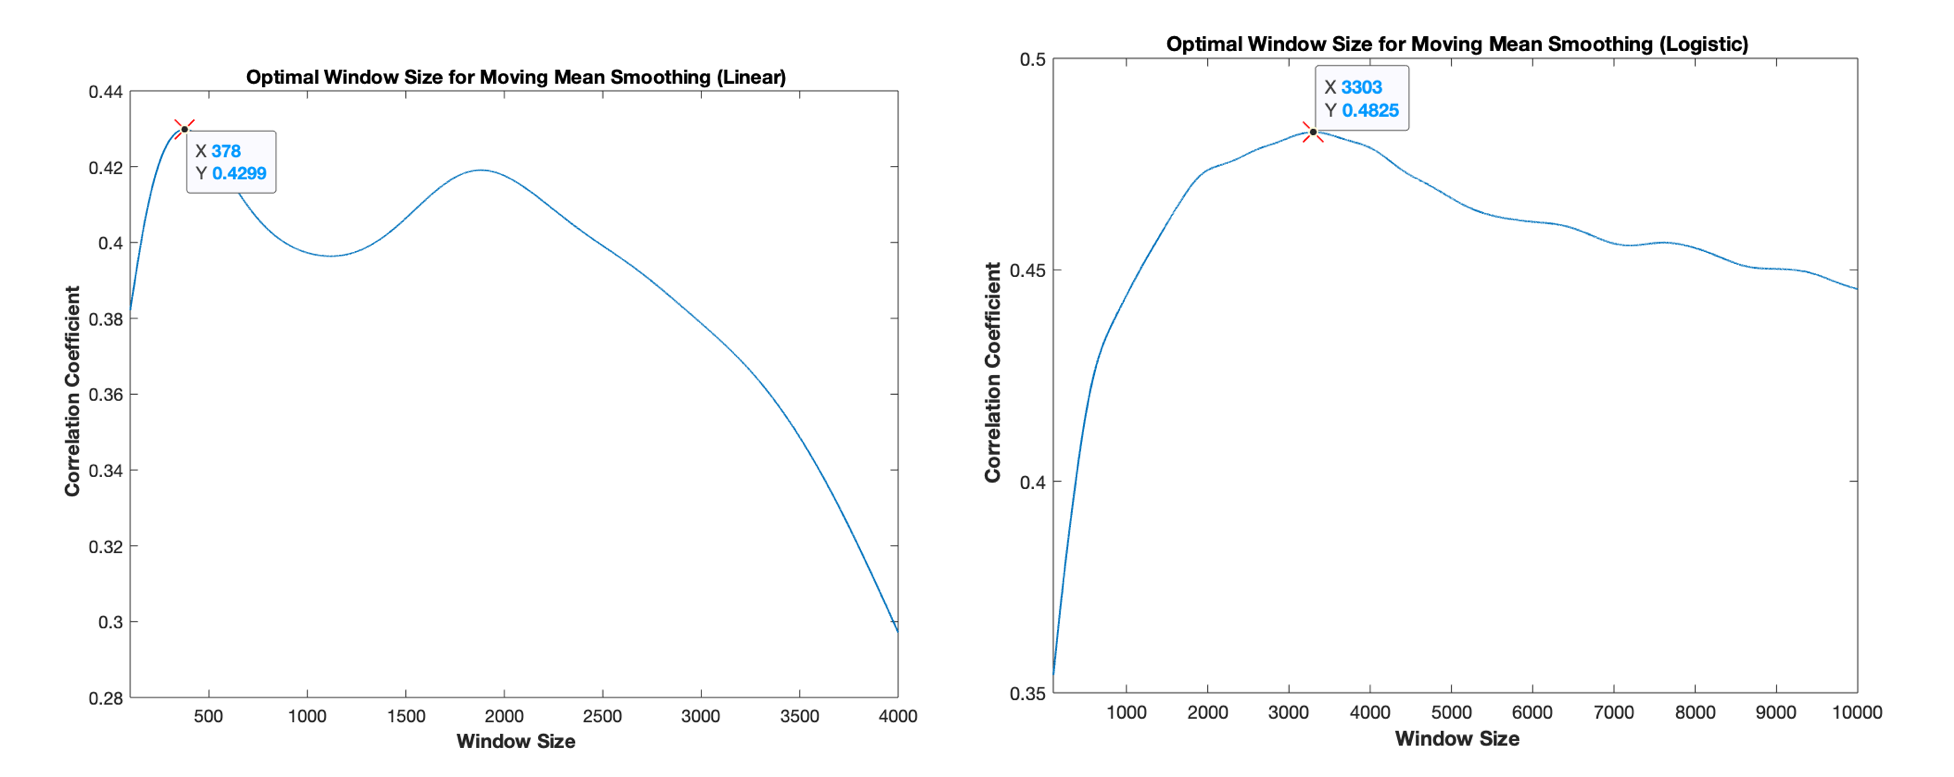
\includegraphics[scale=0.5]{groupwindow.png}
	    \captionof{figure}{Moving average window selection.}
	    \label{fig2}
	\end{minipage}
	
		\begin{minipage}{\linewidth}
        \centering
	    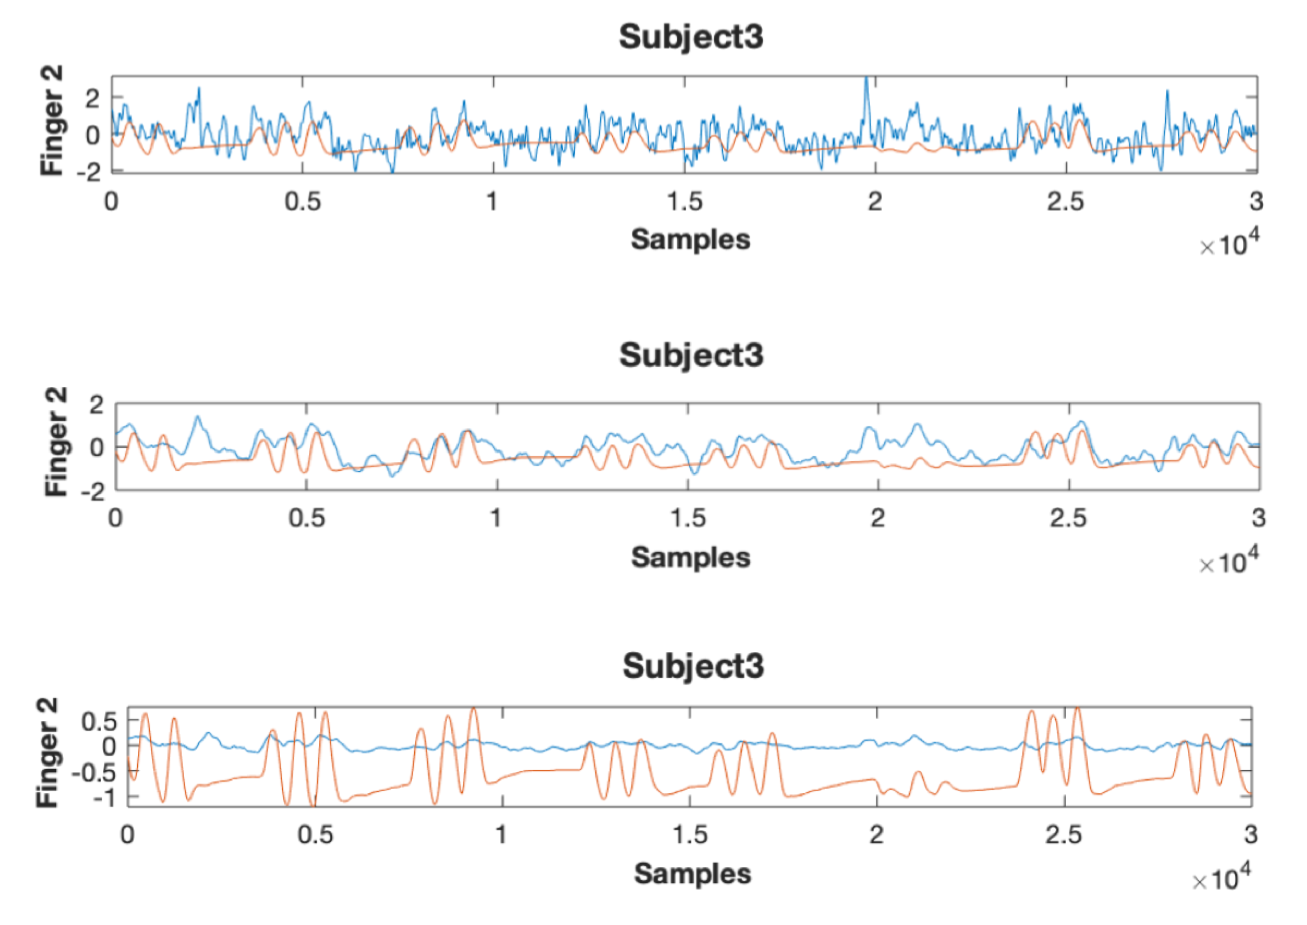
\includegraphics[scale=0.6]{groupdsignals.png}
	    \captionof{figure}{Noisy predictions, smoothed, final}
	    \label{fig3}
	\end{minipage}\\\\
		\begin{minipage}{\linewidth}
        \centering
	    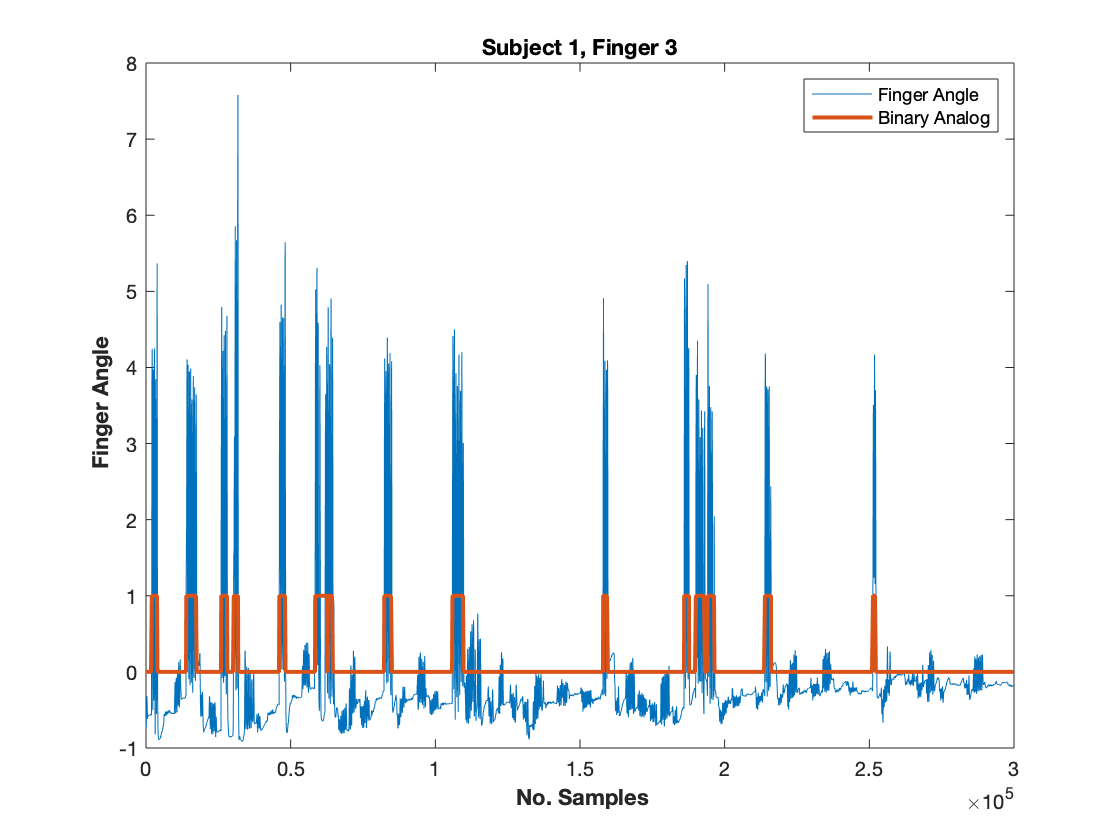
\includegraphics[scale=0.31]{binary_example.png}
	    \captionof{figure}{Smoothed finger angle labels after classifying label as flexion, or non-flexion.}
	    \label{fig4}
	\end{minipage}\\
	
		\begin{minipage}{\linewidth}
        \centering
	    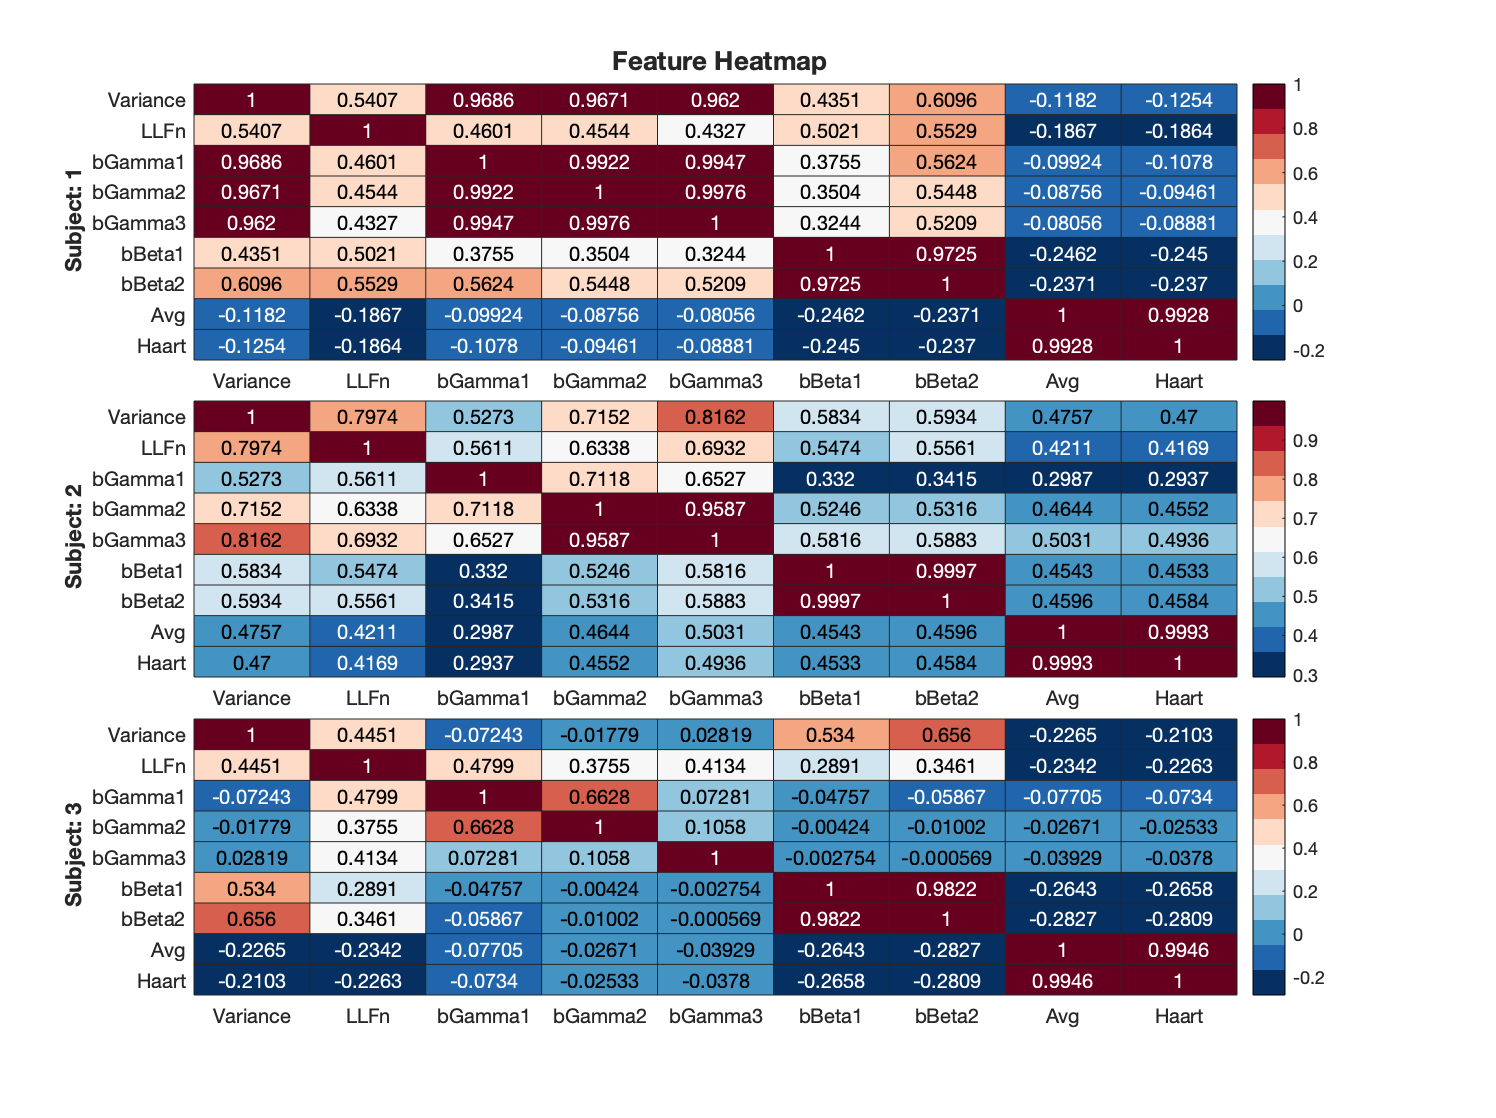
\includegraphics[scale=0.28]{heatmap.png}
	    \captionof{figure}{Feature correlation matrix. Features with co-linearity were removed through trial and error.}
	    \label{fig5}
	\end{minipage}\\\\\\
	
\newpage
\begin{thebibliography}{}
\bibitem{chen} 
Chen, Weixuan, et. Al. “Logistic-Weighted Regression Improves Decoding of Finger Flexion from Electrocorticographic Signals.” Conference proceedings : ... Annual International Conference of the IEEE Engineering in Medicine and Biology Society. IEEE Engineering in Medicine and Biology Society. Annual Conference. U.S. National Library of Medicine, 2014. https://www.ncbi.nlm.nih.gov/pubmed/25570530

\bibitem{hager}
Häger-Ross, C, and M H Schieber. “Quantifying the Independence of Human Finger Movements: Comparisons of Digits, Hands, and Movement Frequencies.” The Journal of neuroscience : the official journal of the Society for Neuroscience. Society for Neuroscience, November 15, 2000. https://www.ncbi.nlm.nih.gov/pubmed/11069962.

\bibitem{kubanek}
Kubánek, J, et. Al. “Decoding Flexion of Individual Fingers Using Electrocorticographic Signals in Humans.” Journal of neural engineering. U.S. National Library of Medicine, December 2009. https://www.ncbi.nlm.nih.gov/pubmed/19794237.

\bibitem{warland}
Warland, D K, and et. Al. “Decoding Visual Information from a Population of Retinal Ganglion Cells.” Journal of neurophysiology. U.S. National Library of Medicine, November 1997. https://www.ncbi.nlm.nih.gov/pubmed/9356386.

\end{thebibliography}
\newpage
\textbf{APPENDIX}\\
	\textbf{Main Script for Model Validation}
	\begin{lstlisting}
		%% (1) Final Project Part 2 (Ikenna Achilihu)
		close all;
		clc;

		% Load raw ECoG data and ECoG test data
		load('raw_training_data.mat', 'train_dg', 'train_ecog');
		load('leaderboard_data.mat', 'leaderboard_ecog');
		% Partiiton fraction for model validation
		frac = 0.9;
		% Sampling freqneucy
		Fs = 1000;
		% Window Length
		win_len = 0.08;
		% Window overlap
		win_lap = 0.04;
		% Number of windows
		num_win = 3;
		% Number of features
		no_feats = 9;

		%% Uncomment for Training Feature Heatmap Creation
		%%%%%%%%%%%%%%%%%%%%%%%%%%%%%%%%%%%%%%%%%%%%%%%%%%%%%%%%%%%%%%%%%%%%%%%%%%%
		subj_trainfeatsHeat = trainfeatsHeat(train_ecog, frac, Fs, win_len, win_lap, no_feats);
		%%%%%%%%%%%%%%%%%%%%%%%%%%%%%%%%%%%%%%%%%%%%%%%%%%%%%%%%%%%%%%%%%%%%%%%%%%%

		%% Uncomment for Feature Heatmap Visualization
		%%%%%%%%%%%%%%%%%%%%%%%%%%%%%%%%%%%%%%%%%%%%%%%%%%%%%%%%%%%%%%%%%%%%%%%%%%%
		xvalues = {'Variance','LLFn','bGamma1','bGamma2','bGamma3','bBeta1','bBeta2','Avg','Haart'};
		yvalues = {'Variance','LLFn','bGamma1','bGamma2','bGamma3','bBeta1','bBeta2','Avg','Haart'};
		visualizeFeats(train_ecog, xvalues, yvalues, subj_trainfeatsHeat);
		%%%%%%%%%%%%%%%%%%%%%%%%%%%%%%%%%%%%%%%%%%%%%%%%%%%%%%%%%%%%%%%%%%%%%%%%%%%

		%% (2) Uncomment for R matrix Creation from Training Data
		%%%%%%%%%%%%%%%%%%%%%%%%%%%%%%%%%%%%%%%%%%%%%%%%%%%%%%%%%%%%%%%%%%%%%%%%%%%
		[trainRmat, mean_trainF, std_trainF] = rMatTrain(train_ecog, frac, Fs, win_len, win_lap, 
		num_win, no_feats);
		%%%%%%%%%%%%%%%%%%%%%%%%%%%%%%%%%%%%%%%%%%%%%%%%%%%%%%%%%%%%%%%%%%%%%%%%%%%

		%% (3) Uncomment for R matrix Creation from Testing Data
		%%%%%%%%%%%%%%%%%%%%%%%%%%%%%%%%%%%%%%%%%%%%%%%%%%%%%%%%%%%%%%%%%%%%%%%%%%%
		testRmat = rMatTest(train_ecog, frac, Fs, win_len, win_lap, num_win, no_feats, mean_trainF, std_trainF);
		%%%%%%%%%%%%%%%%%%%%%%%%%%%%%%%%%%%%%%%%%%%%%%%%%%%%%%%%%%%%%%%%%%%%%%%%%%%

		%% (4) Uncomment to Generate Principle Component Scores
		%%%%%%%%%%%%%%%%%%%%%%%%%%%%%%%%%%%%%%%%%%%%%%%%%%%%%%%%%%%%%%%%%%%%%%%%%%%
		[princ_comp, sc_train, sc_test] = vis_pcafeats(trainRmat, testRmat);
		%%%%%%%%%%%%%%%%%%%%%%%%%%%%%%%%%%%%%%%%%%%%%%%%%%%%%%%%%%%%%%%%%%%%%%%%%%%

		%% (5) Uncomment to Compute Predicitons with Optimal Linear Decoder
		%%%%%%%%%%%%%%%%%%%%%%%%%%%%%%%%%%%%%%%%%%%%%%%%%%%%%%%%%%%%%%%%%%%%%%%%%%%
		[predictions, dg_Test] = optlinDecode(leaderboard_ecog, train_dg, frac, sc_train, sc_test, princ_comp);
		%%%%%%%%%%%%%%%%%%%%%%%%%%%%%%%%%%%%%%%%%%%%%%%%%%%%%%%%%%%%%%%%%%%%%%%%%%%

		%% Lasso Test
		testlassoMod(leaderboard_ecog, train_dg, frac, sc_train, sc_test, princ_comp);
		%% (6) Uncomment to Determine Optimal Paramter for Smoothing Predictions
		%%%%%%%%%%%%%%%%%%%%%%%%%%%%%%%%%%%%%%%%%%%%%%%%%%%%%%%%%%%%%%%%%%%%%%%%%%%
		[opt_Len, opt_Len_fing] = optmovMean(predictions, dg_Test);
		%%%%%%%%%%%%%%%%%%%%%%%%%%%%%%%%%%%%%%%%%%%%%%%%%%%%%%%%%%%%%%%%%%%%%%%%%%%

		%% (7) Uncomment to Smooth Predictions
		%%%%%%%%%%%%%%%%%%%%%%%%%%%%%%%%%%%%%%%%%%%%%%%%%%%%%%%%%%%%%%%%%%%%%%%%%%%
		smooth_Pred = smoothPred(predictions, opt_Len);
		%%%%%%%%%%%%%%%%%%%%%%%%%%%%%%%%%%%%%%%%%%%%%%%%%%%%%%%%%%%%%%%%%%%%%%%%%%%

		%% (8) Uncomment to Classify Finger Data as Action/non-action State
		%%%%%%%%%%%%%%%%%%%%%%%%%%%%%%%%%%%%%%%%%%%%%%%%%%%%%%%%%%%%%%%%%%%%%%%%%%%
		finger_description = classifyFinger(train_dg);
		%%%%%%%%%%%%%%%%%%%%%%%%%%%%%%%%%%%%%%%%%%%%%%%%%%%%%%%%%%%%%%%%%%%%%%%%%%%

		%% (9) Uncomment to Smooth Finger Data States
		%%%%%%%%%%%%%%%%%%%%%%%%%%%%%%%%%%%%%%%%%%%%%%%%%%%%%%%%%%%%%%%%%%%%%%%%%%%
		smoothdg_descrip = smoothfingerStates(finger_description);
		%%%%%%%%%%%%%%%%%%%%%%%%%%%%%%%%%%%%%%%%%%%%%%%%%%%%%%%%%%%%%%%%%%%%%%%%%%%

		%% (10) Uncomment to Generate Finger State Predictions
		%%%%%%%%%%%%%%%%%%%%%%%%%%%%%%%%%%%%%%%%%%%%%%%%%%%%%%%%%%%%%%%%%%%%%%%%%%%
		log_pred = logfingModel(leaderboard_ecog, frac, sc_train, sc_test, smoothdg_descrip, princ_comp);
		%%%%%%%%%%%%%%%%%%%%%%%%%%%%%%%%%%%%%%%%%%%%%%%%%%%%%%%%%%%%%%%%%%%%%%%%%%%

		%% (11) Uncomment to Determine Optimal Paramter for Smoothing Finger States
		%%%%%%%%%%%%%%%%%%%%%%%%%%%%%%%%%%%%%%%%%%%%%%%%%%%%%%%%%%%%%%%%%%%%%%%%%%%
		opt_lenLog = optmovMeanLog(log_pred, smooth_Pred, dg_Test);
		%%%%%%%%%%%%%%%%%%%%%%%%%%%%%%%%%%%%%%%%%%%%%%%%%%%%%%%%%%%%%%%%%%%%%%%%%%%

		%% (12) Uncomment to Smooth Finger State Predictions
		%%%%%%%%%%%%%%%%%%%%%%%%%%%%%%%%%%%%%%%%%%%%%%%%%%%%%%%%%%%%%%%%%%%%%%%%%%%
		smooth_logPred = smoothPred(log_pred, opt_lenLog);
		%%%%%%%%%%%%%%%%%%%%%%%%%%%%%%%%%%%%%%%%%%%%%%%%%%%%%%%%%%%%%%%%%%%%%%%%%%%
		 
		%% (13) Uncomment to Final Compute Logistic-Weighted Predictions
		%%%%%%%%%%%%%%%%%%%%%%%%%%%%%%%%%%%%%%%%%%%%%%%%%%%%%%%%%%%%%%%%%%%%%%%%%%%
		final_Pred = finalPred(smooth_logPred, smooth_Pred);
		%%%%%%%%%%%%%%%%%%%%%%%%%%%%%%%%%%%%%%%%%%%%%%%%%%%%%%%%%%%%%%%%%%%%%%%%%%%

		%% Confirm Prediction Estimates
		%%%%%%%%%%%%%%%%%%%%%%%%%%%%%%%%%%%%%%%%%%%%%%%%%%%%%%%%%%%%%%%%%%%%%%%%%%%
		test(:,1) = diag(corr(final_Pred{1}, dg_Test{1}));
		test(:,2) = diag(corr(final_Pred{2}, dg_Test{2}));
		test(:,3) = diag(corr(final_Pred{3}, dg_Test{3})); 
		mean(mean(test))
		%%%%%%%%%%%%%%%%%%%%%%%%%%%%%%%%%%%%%%%%%%%%%%%%%%%%%%%%%%%%%%%%%%%%%%%%%%%

		%% Uncomment to Visualize Predictions against Finger Test Data
		%%%%%%%%%%%%%%%%%%%%%%%%%%%%%%%%%%%%%%%%%%%%%%%%%%%%%%%%%%%%%%%%%%%%%%%%%%%
		visualizePred(final_Pred, train_dg, frac);
		%%%%%%%%%%%%%%%%%%%%%%%%%%%%%%%%%%%%%%%%%%%%%%%%%%%%%%%%%%%%%%%%%%%%%%%%%%%
	\end{lstlisting}

	\textbf{Functions Used in Model Validation}\\

	\begin{lstlisting}
		function [features] = get_featuresHeat(clean_data,fs)
		%
		% get_featuresHeat.m
		%
		% Instructions: Write a function to calculate features.
		%               Please create 4 OR MORE different features for each channel.
		%               Some of these features can be of the same type (for example, 
		%               power in different frequency bands, etc) but you should
		%               have at least 2 different types of features as well
		%               (Such as frequency dependent, signal morphology, etc.)
		%               Feel free to use features you have seen before in this
		%               class, features that have been used in the literature
		%               for similar problems, or design your own!
		%
		% Input:    clean_data: (samples x channels)
		%           fs:         sampling frequency
		%           
		% Output:   features:   (1 x (channels*features))
		% 
		%% Your code here (8 points)
		% Line Length is function 'LLFn' below

		% Signal Energy
		Energy = @(x) sum(x.^2);

		% Signal Area
		Area = @(x) sum(abs(x));

		% Signal Envelope is function 'sEnvelop' below

		% Average bandpower at Beta and high Gamma range
		bBeta1 = @(x) bandpower(x,fs,[5 15]);
		bBeta2 = @(x) bandpower(x,fs,[20 25]);
		bGamma1 = @(x) bandpower(x,fs,[75 115]);
		bGamma2 = @(x) bandpower(x,fs,[125 160]);
		bGamma3 = @(x) bandpower(x,fs,[160 175]);

		% Average signal power
		pRMS = @(x) rms(x).^2;

		% Average signal value
		avgVal = @(x) mean(x);

		% Relative power at high Gamma range
		RbP = @(x) bandpower(x,fs,[75 115])./rms(x).^2;

		% Spike density is function 'sDen' below

		% Haart wavelet
		haart_ecog = @(x) haart(x);

		% Z-score normalize features
		features = [mean(var(clean_data)) mean(LLFn(clean_data)) ...
		mean(bGamma1(clean_data)) mean(bGamma2(clean_data)) mean(bGamma3...
		(clean_data)) mean(bBeta1(clean_data)) mean(bBeta2(clean_data)) ...
		mean(avgVal(clean_data)) mean(mean(haart_ecog(clean_data)))];
		end
	\end{lstlisting}

	\begin{lstlisting}
		function [all_feats]=getWindowedFeatsHeat(raw_data, fs, window_length, window_overlap, no_features)
		%
		% getWindowedFeatsHeat.m
		%
		% Instructions: Write a function which processes data through the steps
		%               of filtering, feature calculation, creation of R matrix
		%               and returns features.
		%
		%               Points will be awarded for completing each step
		%               appropriately (note that if one of the functions you call
		%               within this script returns a bad output you won't be double
		%               penalized)
		%
		%               Note that you will need to run the filter_data and
		%               get_features functions within this script. We also 
		%               recommend applying the create_R_matrix function here
		%               too.
		%
		% Inputs:   raw_data:       The raw data for all patients
		%           fs:             The raw sampling frequency
		%           window_length:  The length of window
		%           window_overlap: The overlap in window
		%
		% Output:   all_feats:      All calculated features
		%
		%% Your code here (3 points)
		% First, filter the raw data
		new_data = filter_data(raw_data);

		% Sliding window function (Modified for final project)
		NumWins = @(xLen, fs, winLen, winDisp) ((xLen/fs)-winLen+winDisp)/(winDisp); 

		% Compute number of windows and create feature vector
		num_windows = round(NumWins(size(new_data,1), fs, window_length,...
		window_length-window_overlap));

		% Calculate feature descriptor of first window
		winDisp = (window_length-window_overlap)*fs;
		idx = 1:1:(window_length*fs);

		% Initialize feature vector
		all_feats = zeros(num_windows, no_features);

		% Process feature for first window
		all_feats(1,:) = get_featuresHeat(new_data(idx,:), fs);

		% Upper/lower bound for each window
		lower = 1 + winDisp;
		upper = (window_length*fs) + winDisp;

		% Iterate through remaining windows
		for win = 2:num_windows
		    % Compute feature descriptor of every window
		    idx = lower:1:upper;
		    all_feats(win,:) = get_featuresHeat(new_data(idx,:), fs);
		    lower = lower + winDisp;
		    upper = upper + winDisp;
		end
		end
	\end{lstlisting}
	
	\begin{lstlisting}
		function visualizeFeats(ecog, x, y, subj_trainfeatsHeat)
		%
		% visualizeFeats.m
		%
		% Instructions: Function that visualizes normalized feature correlations 
		%               matrix as heatmap. Must pass in ecog data from 
		%               raw_training_data.mat.
		%
		% Input:    ecog:       3x1 Raw ECoG data
		%           x:          nx1 cell array of feature names
		%           y:          nx1 cell array of feature names
		%           
		% Output:   None:       ...
		% 
		%% Code here
		close all
		figure
		plots = tiledlayout(3,1);

		% Iterate through all three subjects
		 for subj = 1:size(ecog,1)
		    %%%%%%%%%%%%%%%%%%%%% Compute heatmap %%%%%%%%%%%%%%%%%%%%%%%%
		    % Create feature correlation matrix for each subject
		    nexttile
		    heatmap(x, y, corr(zscore(subj_trainfeatsHeat{subj})), 'Colormap',redbluecmap);
		    ylabel(['\bf Subject: ', num2str(subj)]);
		 end
		 % Format plot
		 title(plots, '\bf Feature Heatmap');
		 plots.TileSpacing = 'compact';
		end
	\end{lstlisting}

	\begin{lstlisting}
		function [subj_trainRmat, mean_trainFeats, std_trainFeats] = rMatTrain(train_ecog,frac, f, winlen, 
		winlap, numwin, no_feats)
		%
		% rMatTrain.m
		%
		% Instructions: Function computes R feature matrix to use in linear
		% regression.
		%
		% Input:    f:          Smapling frequency
		%           frac:       Partition fractio for training data
		%           train_ecog: 3x1 Raw ECoG data
		%           winlen:     Window length
		%           winlap:     Window overlap
		%           numwin:     No. windows
		%           
		% Output:   subj_trainRmat:     3x1 cell R matrix for training data.
		% 
		%% Code Here
		% Container to store R matrices
		subj_trainRmat = cell(length(train_ecog),1);

		mean_trainFeats = cell(3,1);
		std_trainFeats = cell(3,1);

		%Iterate through all subjects
		for subj = 1:size(train_ecog,1)
		    %%%%%%%%%%%%%%%%% Extract dataglove and ECoG data %%%%%%%%%%%%%%%%%%%%%
		    % ECoG and finger data
		    subj_ecog = train_ecog{subj};
		    
		    % Partition ECoG data
		    ecog_Train = subj_ecog(1:length(subj_ecog)*frac,:);
		    %%%%%%%%%%%%%%%%%%%%%%% Generate R matrices %%%%%%%%%%%%%%%%%%%%%%%%%%%
		    % R training matrix 
		    subj_trainFeats = getWindowedFeats(ecog_Train, f, winlen, winlap, no_feats);
		    % Save statistics for use in test features
		    mean_trainFeats{subj} = mean(subj_trainFeats,1);
		    std_trainFeats{subj} =  std(subj_trainFeats,0,1);
		    subj_trainRmat{subj} = create_R_matrix(zscore(subj_trainFeats), numwin);
		end
		end
	\end{lstlisting}

	\begin{lstlisting}
function subj_testRmat = rMatTest(train_ecog, frac, f, winlen, winlap, numwin, no_feats, mean_trainR, 
std_trainR)
		%
		% rMat.m
		%
		% Instructions: Function computes R feature matrix to use in linear
		% regression.
		%
		% Input:    f:          Smapling frequency
		%           frac:       Partition fractio for training data
		%           train_ecog: 3x1 Raw ECoG data
		%           winlen:     Window length
		%           winlap:     Window overlap
		%           numwin:     No. windows
		%           
		% Output:   subj_testRmat:      3x1 cell R matrix for testing data.
		% 
		%% Code Here
		% Container to store R matrices
		subj_testRmat = cell(length(train_ecog),1);

		%Iterate through all subjects
		for subj = 1:size(train_ecog,1)
		    %%%%%%%%%%%%%%%%% Extract dataglove and ECoG data %%%%%%%%%%%%%%%%%%%%%
		    % ECoG and finger data
		    subj_ecog = train_ecog{subj};  
		    
		    % Partition ECoG data
		    if frac < 1
		        ecog_Test = subj_ecog(length(subj_ecog)*frac+1:end,:);
		    end
		    % Dealing with leaderboard data
		    if frac == 1
		        ecog_Test = subj_ecog;
		    end
		    %%%%%%%%%%%%%%%%%%%%%%% Generate R matrices %%%%%%%%%%%%%%%%%%%%%%%%%%%
		    % R test matrix 
		    subj_testFeats = getWindowedFeats(ecog_Test, f, winlen, winlap, no_feats);
		    
		    % Normalize test features by training features then compute R matrix
		    for col = 1:size(subj_testFeats,2)
		        subj_testFeats(:,col) = (subj_testFeats(:,col) - mean_trainR{subj}(col))/...
		        (std_trainR{subj}(col));
		    end
		    subj_testRmat{subj} = create_R_matrix(subj_testFeats, numwin);  
		end
		end
	\end{lstlisting}

	\begin{lstlisting}
		function [comp, s_train, s_test] = vis_pcafeats(train_R,test_R)
	    %
	    % vis_pcafeats.m
	    %
	    % Instructions: Function that computes optimal principle compenents and
	    % features cast in principle component space.
	    %
	    % Input:    train_R:    3x1 cell R-matrix training features
	    %           test_R:     3x1 cell R-matrix test features
	    %
	    % Output:   s_train:    3x1 cell matrix of principle component features
	    %                       from training data
	    %           s_test:     3x1 cell matrix of principle component features
	    %                       from test data
	    %           comp:       3x1 vector of principle component scores per
	    %                       subject
		%% Code Here
		% Contianers for training/testing scores
		s_train = cell(3,1);
		s_test = cell(3,1);
		% Cutt-off for variance explained
		var_exp = 99;
		% Principle component values
		comp = zeros(size(train_R,1),1);

		close all
		figure
		p1 = tiledlayout(1,3);

		for subj = 1:size(train_R,1)
		    nexttile;
		    % Compute pca statistics on features for every subject
		    [coeff, s_train{subj}, ~, ~, exp_train, mu] = pca(train_R{subj});
		    plot(cumsum(exp_train)*0.01,  'LineWidth', 1); 
		    
		    % Clean up variance explained
		    exp_train = round(cumsum(exp_train));
		    
		    % Extract index (Important principle compnent) 
		    mask = 1:length(exp_train);
		    idx = mask(exp_train == var_exp);
		    comp(subj,1) = idx(1);
		    
		    % Line of most variance
		    hold on;
		    plot(idx(1),99*0.01, '-xr', 'LineWidth', 1, 'MarkerSize', 15);
		    xlim([0 length(exp_train)]);
		    ylim([0 1.2]);
		    
		    % Construct scores for testing features
		    s_test{subj} = (test_R{subj} - repmat(mu,size(test_R{subj},1),1))/coeff';
		end
		% Format plot
		xlabel(p1,'\bf Principle Component');
		ylabel(p1,'\bf Cummulative Variance Explained');
		title(p1, '\bf Components Needed to Explain Variance (Train)');
		p1.TileSpacing = 'compact';
		end
	\end{lstlisting}

	\begin{lstlisting}
		function [pred, dg_Test] = optlinDecode(leader, train_dg, frac, subj_trainRmat, subj_testRmat, pc)
	    %
	    % optlinDecode.m
	    %
	    % Instructions: Function that computes feature predictions and
	    % correlation coefficients using optimal linear decoder algorithm
	    %
	    % Input:    train_dg:   3x1 raw finger data
	    %           frac:       Partition fraction
	    %
	    % Output:   pred:       Angle predictions
	    %           dg_Test:    3x1 Cell finger test data
		%% Code Here
		% Container for finger test data
		dg_Test = cell(3,1);
		% Container for predictions
		pred = cell(3,1);

		%Iterate through all subjects
		for subj = 1:size(train_dg,1)
		    %%%%%%%%%%%%%%%%% Extract dataglove and ECoG data %%%%%%%%%%%%%%%%%%%%%
		    % Finger data
		    subj_dg = train_dg{subj};
		    
		    % Partition finger position
		    dg_Train = subj_dg(1:length(subj_dg)*frac,:);
		    
		    % Dealing with partition of training data as test data
		    if frac < 1
		        dg_Test{subj} = subj_dg(length(subj_dg)*frac+1:end,:);
		    end
		    % Dealing with leaderboard data as testing data
		    if frac == 1
		        dg_Test{subj} = leader{subj};
		    end
		    %%%%%%%%%%% Angle predictions using optimal linear decoding %%%%%%%%%%%
		    % Downsample training finger data, delete extra row 
		    dg_Train = downsample(dg_Train, round(size(dg_Train,1)/size(subj_trainRmat{subj}...
		    (:,1:pc(subj)),1)));
		    dg_Train = dg_Train(1:(end-1),:);
		    
		    % Calculate f matrix for 5 fingers using equation (1)
		    f_Mat = mldivide(subj_trainRmat{subj}(:,1:pc(subj))'*subj_trainRmat{subj}(:,1:pc(subj)),...
		    (subj_trainRmat{subj}(:,1:pc(subj))'*dg_Train));
		    
		    % Generate finger predictions
		    subj_pred = subj_testRmat{subj}(:,1:pc(subj))*f_Mat;
		    
		    % Upsample prediction vector
		    subj_pred =  resample(subj_pred, round(size(dg_Test{subj},1)/size(subj_pred,1)),1);
		    
		    % Create vector of extrapolated points by mean of previous n samples 
		    vect = repmat(mean(subj_pred(size(subj_pred,1)-(size(dg_Test{subj},1)-...
		        size(subj_pred,1))+1:end,:)), size(dg_Test{subj},1)-size(subj_pred,1),1);
		    
		    % Finalze finger angle prediction vector and store
		    pred{subj} = [subj_pred; vect];    
		end
		end
	\end{lstlisting}

	\begin{lstlisting}
		function testlassoMod(leader, train_dg, frac, subj_trainRmat, subj_testRmat, pc)

		% Container for finger test data
		dg_Test = cell(3,1);

		% Container for predictions
		pred = cell(3,1);

		lin_decCorr = zeros(5,3);

		% Iterate through all alpha parameters
		alpha = 0.01:0.1:1;
		% Container to store correlation coefficients
		c = zeros(1,length(alpha));
		i = 0;
		for k = 1:length(alpha)
		    i = i+1;
		    %%%%%%%%%%%%%%%%% Extract dataglove and ECoG data %%%%%%%%%%%%%%%%%%%%%
		    %Iterate through all subjects
		    for subj = 1:size(train_dg,1)
		        % Finger data
		        subj_dg = train_dg{subj};
		        
		        % Partition finger position
		        dg_Train = subj_dg(1:length(subj_dg)*frac,:);
		        
		       % Dealing with partition of training data as test data
		       if frac < 1
		           dg_Test{subj} = subj_dg(length(subj_dg)*frac+1:end,:);
		       end
		       % Dealing with leaderboard data as testing data
		       if frac == 1
		           dg_Test{subj} = leader{subj};
		       end
		      %%%%%%%%%%%%%%%%%%%% Generate finger state model %%%%%%%%%%%%%%%%%%%% 
		       % Downsample training finger data, delete extra row 
		       dg_Train = downsample(dg_Train, round(size(dg_Train,1)/size(subj_trainRmat{subj}(:,...
		       1:pc(subj)),1)));
		       dg_Train = dg_Train(1:(end-1),:);
		       
		       for fing = 1:size(train_dg{subj},2)
		           %Train model on training data on current finger
		           [B,FitInfo] = lasso(subj_trainRmat{subj}(:,1:pc(subj)),dg_Train(:,fing),'Alpha',...
		           alpha(k), 'CV',5);
		           idxLambda1SE = FitInfo.Index1SE;
		           coef = B(:,idxLambda1SE);
		           coef0 = FitInfo.Intercept(idxLambda1SE);
		            
		            %Predict finger states
		            yhat = subj_testRmat{subj}(:,1:pc(subj))*coef + coef0;
		            
		            % Upsample prediction vector
		            yhat = resample(yhat, round(size(dg_Test{subj},1)/size(yhat,1)),1);
		            
		            % Create vector of extrapolated points by mean of previous n
		            vect = repmat(mean(yhat(size(yhat,1)-(size(dg_Test{subj},1)-...
		            size(yhat,1))+1:end,:)), size(dg_Test{subj},1)-size(yhat,1),1);
		            
		            % Finalze finger state prediction vector and store
		            pred{subj}(:,fing) = [yhat; vect];
		       end
		       % Correlation values
		       lin_decCorr(:,subj) = diag(corr(pred{subj}, dg_Test{subj})); 
		       
		    end
		    % Vector of correlation coefficients
			c(i) = mean(mean(lin_decCorr));
		end

		% Optimal alpha 
		[~,idx] = max(c);
		opt_alpha = alpha(idx);

		%% Plot output
		close all
		figure

		plot(alpha, c, 'LineWidth', 1);
		hold on;
		plot(opt_alpha,max(c), '-xr', 'LineWidth', 1, 'MarkerSize', 15);
		hold off;

		% Format plot
		xlim([min(alpha) max(alpha)]);
		xlabel('\bf Alpha Parameter');
		ylabel('\bf Correlation Coefficient');
		title('\bf Optimal Alpha Size');

		end
	\end{lstlisting}

	\begin{lstlisting}
		function [opt_winLen, opt_winLen_fing] = optmovMean(pred, dg_Test)
	    %
	    % optmovMean.m
	    %
	    % Instructions: Function that computes optimal window length for moving
	    % average smoothing across all subjects
	    %
	    % Input:    pred:       Unfiltered predictions
	    %           dg_Test:    3x1 cell test finger data
	    %
	    % Output:   opt_winLen:         Optimal window length
	    %           opt_winLen_fing:    5x1 vector optimal window length per finger
		%% Code here
		% Container to store corrleation coefficients per finger per subject
		lin_decCorr = zeros(size(dg_Test{1},2),size(dg_Test,1));
		% Window size vector
		windowsize = 100:1:4000;
		% Container to store correlation coefficients
		c = zeros(1,length(windowsize));
		% Contianer to store smoothed predictions per finger per subject
		mov_meanFing = zeros(length(windowsize),size(pred{1},2),size(dg_Test,1));
		i = 0;
		for k = 1:length(windowsize)
		    i = i+1;
		    for subj = 1:size(pred,1)
		        % Extract correlation coefficients
		        lin_decCorr(:,subj) = diag(corr(movmean(pred{subj}, windowsize(k)),...
		        dg_Test{subj}));
		        
		        for fing = 1:size(pred{subj},2)
		            % Extract corr. coeff. for all fingers/subjects
		            mov_meanFing(i,fing,subj) = corr(movmean(pred{subj}(:,fing),...
		            windowsize(k)), dg_Test{subj}(:,fing));
		        end        
		    end
		    % Vector of correlation coefficients
			c(i) = mean(mean(lin_decCorr));
		    % Mean correlation coefficients for all fingers across all window sizes
		    c_fing = mean(mov_meanFing,3);
		end
		% Optimal window size
		[~,idx] = max(c);
		opt_winLen = windowsize(idx);
		%% Plot output
		close all
		figure

		plot(windowsize, c, 'LineWidth', 1);
		hold on;
		plot(opt_winLen,max(c), '-xr', 'LineWidth', 1, 'MarkerSize', 15);
		hold off;

		% Format plot
		xlim([min(windowsize) max(windowsize)]);
		xlabel('\bf Window Size');
		ylabel('\bf Correlation Coefficient');
		title('\bf Optimal Window Size for Moving Mean Smoothing (Linear)');
		% legend([coeff win], 'Max correlation coefficient', 'Optimal window size')
		%% Plot output
		figure
		p = tiledlayout(5,1);
		opt_winLen_fing = zeros(5,1);
		for fing = 1:5
		    [~,idx] = max(c_fing(:,fing));
		    opt_winLen_fing(fing) = windowsize(idx);

		    nexttile
		    plot(windowsize, c_fing(:,fing),'LineWidth', 1);
		    xlim([min(windowsize) max(windowsize)]);
		    ylabel(['\bf Finger ',num2str(fing)]);
		    hold on;
		    plot(opt_winLen_fing(fing), max(c_fing(:,fing)), '-xr', 'LineWidth', 1, 'MarkerSize', 15);
		    hold off;
		end
		% Format plot
		xlabel(p,'\bf Window Size');
		ylabel(p,'\bf Correlation Coefficient');
		title(p,'\bf Optimal Window Size for Moving Mean Smoothing - by Finger');

		%Save optimal window length value
		save('opt_winLen.mat', 'opt_winLen');
		end
	\end{lstlisting}

	\begin{lstlisting}
		function new_pred = smoothPred(pred,len)
	    %
	    % smoothPred.m
	    %
	    % Instructions: Function that computes movine mean smoothing of
	    % predictions using optimal window length.
	    %
	    % Input:    pred:       3x1 cell array of unfiltered predictions
	    %           len:        Optimal window length
	    %
	    % Output:   new_pred:   3x1 cell array of filtered predictions
	    % 
		%% Code Here
		% Initialize container for filtered predictions
		new_pred = cell(3,1);
		for subj = 1:size(pred,1)
		    % Apply moving mean to predictions for all subjects and fingers
		    new_pred{subj} = movmean(pred{subj}, len);
		end
		end
	\end{lstlisting}

	\begin{lstlisting}
		function dg_descrip = classifyFinger(dg)
	    %
	    % classifyFinger.m
	    %
	    % Instructions: Function that classifies fingers angles as motion,
	    % no-motion based on a threshold angle
	    %
	    % Input:    dg:         3x1 cell array of finger angles
	    %
	    % Output:   dg_descrip: 3x1 cell array of finger states
		%% Code Here
		% Container for finger threshold
		dg_descrip = cell(3,1);
		% Threshold for finger data
		thresh = 1.5;

		for subj = 1:size(dg,1)
		    for fing = 1:size(dg{subj},2)
		        dg_descrip{subj}(:,fing) = dg{subj}(:,fing) >= thresh;
		    end
		end
		end
	\end{lstlisting}

	\begin{lstlisting}
		function dg_descrip = smoothfingerStates(dg_descrip)
	    %
	    % smoothfingerStates.m
	    %
	    % Instructions: Function that smoothes finger states accoring to a
	    % moving window
	    %
	    % Input:    dg_descrip:         3x1 cell array of finger states
	    %
	    % Output:   dg_descrip: 3x1 cell array of smoothed finger states
		%% Code Here
		% Smoothing factor every 4 seconds
		sm = 4000;
		% Iterate through all subject and fingers
		for subj = 1:size(dg_descrip,1)
		    for fing = 1:size(dg_descrip{subj},2) 
		        % Current vector
		        vect = dg_descrip{subj}(:,fing);
		        % Find all peaks
		       [~, idx] = findpeaks(double(dg_descrip{subj}(:,fing)));
		       % Index corresponding to first peak
		       first = idx(1);
		       for i = 1:length(idx) 
		           % Have not reached last pulse train of ones
		           if idx(i) > first+sm 
		               % Last pulse train of ones    
		               last = idx(i-1);
		               % Current range
		               range = first:1:last;
		               vect(range) = 1;
		               first = idx(i);
		           end
		           % Merge last pulse train of ones
		           if idx(i) == idx(end)
		               last = idx(i);
		               range = first:1:last;
		               vect(range) = 1;
		           end
		       end
		       % Update finger vector
		       dg_descrip{subj}(:,fing) = vect;
		    end
		end
		end
	\end{lstlisting}

	\begin{lstlisting}
		function log_pred = logfingModel(leader, frac, train_R, test_R, f_descrip, pc)
	    %
	    % logfingModel.m
	    %
	    % Instructions: Function that generates logistic regression predictions
	    % based on finger state data
	    %
	    % Input:    frac:           Partition fraction
	    %           f_descrip:      3x1 cell of finger state data
	    %           train_R:        3x1 cell matrix of principle component features
	    %                           from training data
	    %           test_R:         3x1 cell matrix of principle component features
	    %                           from test data
	    %           pc:             3x1 vector of principle components for each
	    %                           subject
	    %           leader:         3x1 cell matrix of leaderboard test data
	    % Output:   log_pred:       3x1 cell matrix of logistic predictions
		%% Code Here
		% Container for finger test data
		f_Test = cell(3,1);

		% Container for predictions
		log_pred = cell(3,1);

		%Iterate through all subjects
		for subj = 1:size(f_descrip,1)
		    % Finger descriptions
		    subj_f = f_descrip{subj};
		    
		    % Partition finger descriptions
		    f_Train = subj_f(1:length(subj_f)*frac,:);
		    
		    % Dealing with partition of training data as test data
		    if frac < 1
		        f_Test{subj} = subj_f(length(subj_f)*frac+1:end,:);
		    end
		    % Dealing with leaderboard data as testing data
		    if frac == 1
		        f_Test{subj} = leader{subj};
		    end
		%%%%%%%%%%%%%%%%%%%%%%% Generate finger state model %%%%%%%%%%%%%%%%%%%%%%%
		    % Downsample finger states, delete extra row 
		    f_Train = downsample(f_Train, round(size(f_Train,1)/size(train_R{subj}(:,1:pc(subj)),1)));
		    f_Train = f_Train(1:(end-1),:);
		    
		    for fing = 1:size(f_descrip{subj},2)
		        %Train model on training data
		        mdl = fitglm(train_R{subj}(:,1:pc(subj)), f_Train(:,fing));
		        
		        %Predict finger states
		        prob = predict(mdl, test_R{subj}(:,1:pc(subj)));
		        
		        % Upsample finger state vector
		        prob = resample(prob, round(size(f_Test{subj},1)/size(prob,1)),1);       
		    
		        % Create vector of extrapolated points by mean of previous n 
		        vect = repmat(mean(prob(size(prob,1)-(size(f_Test{subj},1)-...
		            size(prob,1))+1:end,:)), size(f_Test{subj},1)-size(prob,1),1);
		       
		        % Finalze finger state prediction vector and store
		        log_pred{subj}(:,fing) = [prob; vect]; 
		    end
		end
	\end{lstlisting}

	\begin{lstlisting}
		function opt_lenLog = optmovMeanLog(log_pred, smooth_Pred, dg_Test)
	    %
	    % optmovMeanLog.m
	    %
	    % Instructions: Function that computes optimal window length for moving
	    % average smoothing across all subjects for logistic predictions
	    %
	    % Input:    smooth_Pred:        3x1 cell of smoothed predictions
	    %           dg_Test:            3x1 cell test finger data
	    %
	    % Output:   opt_lenLog:         Optimal window length
		%% Code Here
		% Container to store corrleation coefficients per finger per subject
		lin_decCorr = zeros(5,3);
		% Window size vector
		windowsize = 100:1:10000;
		% Container to store correlation coefficients
		c = zeros(1,length(windowsize));
		% Contianer to store smoothed predictions per finger per subject
		mov_meanFing = zeros(length(windowsize),size(dg_Test{1},2),size(dg_Test,1));
		i = 0;
		for k = 1:length(windowsize)
		    i = i+1;
		     for subj = 1:size(log_pred,1)
		         % Extract correlation coefficients
		         lin_decCorr(:,subj) = diag(corr((movmean(log_pred{subj}, windowsize(k))...
		         .* smooth_Pred{subj}),dg_Test{subj})); 
		     
		         for fing = 1:size(dg_Test{1},2)
		             % Extract corr. coeff. for all fingers/subjects
		             mov_meanFing(i,fing,subj) = corr((movmean(log_pred{subj}(:,fing), ...
		             windowsize(k)) .* smooth_Pred{subj}(:,fing)),dg_Test{subj}(:,fing));
		         end
		     end
		     % Vector of correlation coefficients
			c(i) = mean(mean(lin_decCorr));    
		    % Mean correlation coefficients for all fingers across all window sizes
		    c_fing = mean(mov_meanFing,3);
		end
		% Optimal window size
		[~,idx] = max(c);
		opt_lenLog = windowsize(idx);
		%% Plot output
		close all
		figure

		plot(windowsize, c, 'LineWidth', 1);
		hold on;
		plot(opt_lenLog,max(c), '-xr', 'LineWidth', 1, 'MarkerSize', 15);
		hold off;

		% Format plot
		xlim([min(windowsize) max(windowsize)]);
		xlabel('\bf Window Size');
		ylabel('\bf Correlation Coefficient');
		title('\bf Optimal Window Size for Moving Mean Smoothing (Logistic)');

		%Save optimal window length value
		save('opt_lenLog.mat', 'opt_lenLog');

		%% Plot output
		figure
		p = tiledlayout(5,1);
		opt_winLen_fing = zeros(5,1);
		for fing = 1:5
		    [~,idx] = max(c_fing(:,fing));
		    opt_winLen_fing(fing) = windowsize(idx);

		    nexttile
		    plot(windowsize, c_fing(:,fing),'LineWidth', 1);
		    xlim([min(windowsize) max(windowsize)]);
		    ylabel(['\bf Finger ',num2str(fing)]);
		    hold on;
		    plot(opt_winLen_fing(fing), max(c_fing(:,fing)), '-xr', 'LineWidth', 1, 'MarkerSize', 15);
		    hold off;
		end
		% Format plot
		xlabel(p,'\bf Window Size');
		ylabel(p,'\bf Correlation Coefficient');
		title(p,'\bf Optimal Window Size for Moving Mean Smoothing - by Finger');
		end
	\end{lstlisting}

	\begin{lstlisting}
		function final_Pred = finalPred(smooth_logPred, smooth_Pred)
	    %
	    % finalPred.m
	    %
	    % Instructions: Function that weights linear regression results with
	    % logistic regression results according to y = y_{lin}*y_{log} to
	    % produce final predictions
	    %
	    % Input:    smooth_logPred:     Smoothed logistic regression results
	    %           smooth_Pred:        Smoothed linear regression results
	    %
	    % Output:   final_Pred:         Final predictions
		%% Code Here
		final_Pred = cell(3,1);
		for subj = 1:size(smooth_logPred,1)
		    final_Pred{subj} = smooth_logPred{subj}.*smooth_Pred{subj};
		end
		end
	\end{lstlisting}

	\textbf{Script for Competition}\\

	\begin{lstlisting}
		function [predicted_dg] = make_predictions(test_ecog)

		% INPUTS: test_ecog - 3 x 1 cell array containing ECoG for each subject, where test_ecog{i} 
		% to the ECoG for subject i. Each cell element contains a N x M testing ECoG,
		% where N is the number of samples and M is the number of EEG channels.

		% OUTPUTS: predicted_dg - 3 x 1 cell array, where predicted_dg{i} contains the 
		% data_glove prediction for subject i, which is an N x 5 matrix (for
		% fingers 1:5)

		% Run time: The script has to run less than 1 hour. 

		%%%%%%%%%%%%%%%%%%%%%%%%%%%%%%%%%%%%%%%%%%%%%%%%%%%
		%% Code here
		close all;
		clc;

		% Load optimal window length parameter for moving average smoothing
		load('opt_winLen.mat', 'opt_winLen');
		load('opt_lenLog.mat', 'opt_lenLog');
		% Load raw ECoG data and ECoG test data
		load('raw_training_data.mat', 'train_dg', 'train_ecog');
		% Partiiton fraction for model validation
		frac = 1;
		% Sampling freqneucy
		Fs = 1000;
		% Window Length
		win_len = 0.08;
		% Window overlap
		win_lap = 0.04;
		% Number of windows
		num_win = 3;
		% Number of features
		no_feats = 9;

		% Generate training/testing features
		[trainRmat, mean_trainF, std_trainF] = rMatTrain(train_ecog, frac, Fs, win_len, win_lap,...
		 num_win, no_feats);
		testRmat = rMatTest(test_ecog, frac, Fs, win_len, win_lap, num_win, no_feats, mean_trainF,...
		 std_trainF);

		% Use features to generate principle components
		[princ_comp, sc_train, sc_test] = vis_pcafeats(trainRmat, testRmat);

		% Generate linear predictions
		[predictions, ~] = optlinDecode(test_ecog, train_dg, frac, sc_train, sc_test, princ_comp);

		% Smooth linear predictions
		smooth_Pred = smoothPred(predictions, opt_winLen);

		% Classify finger state/non-state data
		finger_description = classifyFinger(train_dg);

		% Smooth finger data states
		smoothdg_descrip = smoothfingerStates(finger_description);

		% Generate finger state predictions
		log_pred = logfingModel(test_ecog, frac, sc_train, sc_test, smoothdg_descrip, princ_comp);

		% Smooth finger state predictions
		smooth_logPred = smoothPred(log_pred, opt_lenLog);

		% Generate final logistic-weighted predictions
		predicted_dg = finalPred(smooth_logPred, smooth_Pred);
		end
	\end{lstlisting}

\end{document}